\id{IRSTI 61.31.57}{}

{\bfseries HYDROGEN STORAGE IN POROUS CARBON MATERIALS OBTAINED BASED ON
KAZAKHSTAN COALS}

{\bfseries \textsuperscript{1,2}M.K.
Kazankapova}
\begin{figure}[H]
	\centering
	
\includegraphics[width=0.8\textwidth]{media/chem2/image1}
	\caption*{}
\end{figure}
{\bfseries \textsuperscript{\envelope },
\textsuperscript{1,2}B.T.Yermagambet}
\begin{figure}[H]
	\centering
	
\includegraphics[width=0.8\textwidth]{media/chem2/image1}
	\caption*{}
\end{figure}
{\bfseries ,
\textsuperscript{1,2}Zh.M.
Kassenova}
\begin{figure}[H]
	\centering
	
\includegraphics[width=0.8\textwidth]{media/chem2/image1}
	\caption*{}
\end{figure}
{\bfseries ,\textsuperscript{1,2}A.B.Malgazhdarova}
\begin{figure}[H]
	\centering
	
\includegraphics[width=0.8\textwidth]{media/chem2/image1}
	\caption*{}
\end{figure}
{\bfseries ,
\textsuperscript{1,3}Zh.T.Dauletzhanova}
\begin{figure}[H]
	\centering
	
\includegraphics[width=0.8\textwidth]{media/chem2/image1}
	\caption*{}
\end{figure}
{\bfseries ,
\textsuperscript{1,2}U.M.
Kozhamuratova}
\begin{figure}[H]
	\centering
	
\includegraphics[width=0.8\textwidth]{media/chem2/image1}
	\caption*{}
\end{figure}
{\bfseries ,
\textsuperscript{1,2}G.
K.Mendaliyev}
\begin{figure}[H]
	\centering
	
\includegraphics[width=0.8\textwidth]{media/chem2/image1}
	\caption*{}
\end{figure}
{\bfseries ,
\textsuperscript{1}A.S.
Akshekina}
\begin{figure}[H]
	\centering
	
\includegraphics[width=0.8\textwidth]{media/chem2/image1}
	\caption*{}
\end{figure}


\textsuperscript{1}«Institute of Coal Chemistry and Technology» LLP,
Astana, Kazakhstan,

\textsuperscript{2}L.N. Gumilyov Eurasian National University,
Astana, Kazakhstan,

\textsuperscript{3}Kazakh university of technology and business named
after K. Kulazhanov, Astana, Kazakhstan

{\bfseries \textsuperscript{\envelope }}Корреспондент-автор: maira\_1986@mail.ru,
\href{mailto:coaltech@bk.ru}{\nolinkurl{coaltech@bk.ru}},

The study is devoted to the investigation of hydrogen sorption
properties of activated carbon adsorbents made of coals from the
Kazakhstan deposits "Shubarkol" and "Shoptykol". To activate the
samples, KOH treatment in a ratio of 1:0.5 was used, followed by thermal
activation at a temperature of 900 °C. The specific surface area of
\hspace{0pt}\hspace{0pt}the samples was determined using the BET method,
and their ability to absorb hydrogen at different temperature conditions
was assessed. The study showed that the largest specific surface area
(926.67 m²/g) and maximum hydrogen sorption capacity (1.48 wt.\%) at a
temperature of 77 K are demonstrated by the powdered adsorbent
"Shoptykol;KOH" (ratio 1:0.5, treatment temperature 900 °C).
Adsorption-desorption isotherms of these materials classify them as type
I and type II, which indicates the mesoporous structure of extruded
adsorbents and the more developed microporous texture of powder analogs.
Temperature studies have revealed that lowering the temperature
increases both the specific surface area and the adsorption capacity for
hydrogen, reaching a peak of sorption at cryogenic temperatures. In this
regard, powdered "Shoptykol:KOH" (1:0.5, 900°C) is recognized as the
optimal material for storing hydrogen due to its high specific surface
area, developed microporous structure and exceptional ability to absorb
hydrogen.

{\bfseries Key words:} coal, adsorbent, porosity, carbonization,
adsorption, hydrogen.

{\bfseries ҚАЗАҚСТАН КӨМІРЛЕРІНЕН АЛЫНҒАН КЕУЕКТІ КӨМІРТЕКТІ МАТЕРИАЛДАРДА
СУТЕКТІ САҚТАУ}

{\bfseries \textsuperscript{1,2}М.Қ. Қазанқапова\textsuperscript{\envelope },
\textsuperscript{1,2}Б.Т.Ермағамбет, \textsuperscript{1,2}Ж.M.
Касенова,\textsuperscript{1,2}А.Б. Малғаждарова,
\textsuperscript{1,3}Ж.Т.Даулетжанова,
\textsuperscript{1,2}Ұ.М.Қожамұратова, \textsuperscript{1,2}Г.К.
Мендалиев, \textsuperscript{1}Ә.С. Акшекина}

\textsuperscript{1}«Көмір химиясы және технология институты» ЖШС,
Астана, Қазақстан,

\textsuperscript{2}Л.Н. Гумилев атындағы Еуразия ұлттық университеті,
Астана, Қазақстан,

\textsuperscript{3}Қ.Құлажанов атындағы қазақ технология және бизнес
университеті, Astana, Kazakhstan,

е-mail: \href{mailto:coaltech@bk.ru}{\nolinkurl{coaltech@bk.ru}},
maira\_1986@mail.ru

Зерттеу Қазақстанның «Шұбаркөл» және «Шоптыкөл» кен орындарының
көмірлерінен алынған белсендірілген көмір адсорбенттерінің сутегіні
сорбциялау қасиеттерін зерттеуге арналған. Үлгілерді белсендіру үшін
1:0,5 қатынасында KOH-мен өңдеу, содан кейін 900 °C температурада
термиялық белсендіру қолданылды. Үлгілердің меншікті бетінің ауданы БЭТ
әдісімен анықталды және олардың сутегін сіңіру қабілеті әртүрлі
температура жағдайында бағаланды. Зерттеу көрсеткендей, ең үлкен
меншікті бетінің ауданы (926,67 м²/г) және сутегінің максималды
сорбциялық қабілеті (1,48 мас.\%) 77 К температурада «Шоптыкөл:KOН»
ұнтақ адсорбентімен (қатынасы 1:0,5, өңдеу температурасы 900 °С)
көрсетілген. Бұл материалдардың адсорбциялық-десорбциялық изотермалары
экструдталған адсорбенттердің мезокеуекті құрылымын және ұнтақ
аналогтарының неғұрлым дамыған микрокеуекті құрылымын көрсете отырып,
оларды I және II типке жатқызылды. Температуралық зерттеулер
температураны төмендету меншікті бетінің ауданын да, сутегінің
адсорбциялық қабілетін де арттырып, криогендік температурада сорбциялық
шыңға жететінін анықтады. Осыған байланысты «Шоптыкөл:КОН» ұнтағы
(1:0,5, 900°С) жоғары меншікті бетінің ауданына, дамыған микрокеуекті
құрылымына және сутекті сіңіру қабілетіне байланысты сутегін сақтау үшін
оңтайлы материал болып танылды.

{\bfseries Түйін сөздер:} көмір, адсорбент, кеуектілік, карбонизация,
адсорбция, сутегі.

{\bfseries ХРАНЕНИЕ ВОДОРОДА В ПОРИСТЫХ УГЛЕРОДНЫХ МАТЕРИАЛАХ ПОЛУЧЕННЫХ НА
ОСНОВЕ УГЛЕЙ КАЗАХСТАНА}

{\bfseries \textsuperscript{1,2}М.К.Казанкапова\textsuperscript{\envelope },
\textsuperscript{1,2}Б.Т Ермағамбет, \textsuperscript{1,2}Ж.M.Касенова,
\textsuperscript{1,2}А.Б. Малғаждарова,}

{\bfseries \textsuperscript{1,3}Ж.Т. Даулетжанова,
\textsuperscript{1,2}Ұ.М.Қожамұратова, \textsuperscript{1,2}Г.К.
Мендалиев, \textsuperscript{1}Ә.С. Акшекина}

\textsuperscript{1}ТОО «Институт химии угля и технологии», Астана,
Казахстан,

\textsuperscript{2}Евразийский национальный университет им. Л.Н.
Гумилева, Астана, Казахстан,

\textsuperscript{3}Казахский университет технологии и бизнеса имени К.
Кулажанова, Астана, Казахстан,

е-mail: \href{mailto:coaltech@bk.ru}{\nolinkurl{coaltech@bk.ru}},
maira\_1986@mail.ru

Исследование посвящено изучению водородосорбционных свойств
активированных углеродных адсорбентов, изготовленных из углей
Казахстанских месторождений «Шубарколь» и «Шоптыколь». Для активирования
образцов использовалась обработка КОН в соотношении 1:0,5, а затем
термическая активация при температуре 900 °С. Определены удельная
поверхность образцов с помощью метода БЭТ, а также проведена оценка их
способности поглощать водород при разных температурных режимах.
Исследование показало, что наибольшую удельную поверхность (926,67 м²/г)
и максимальную водородосорбционную емкость (1,48 мас.\%) при температуре
77 К демонстрирует порошкообразный адсорбент "Шоптыколь;КОН"
(соотношение 1:0,5, температура обработки 900 °С). Изотермы
адсорбции-десорбции этих материалов классифицируют их как тип I и тип
II, что свидетельствует о мезопористой структуре экструдированных
адсорбентов и более развитой микропористой текстуре порошкообразных
аналогов. Температурные исследования выявили, что понижение температуры
повышает как удельную поверхность, так и адсорбционную способность к
водороду, достигая пика сорбции при криогенных температурах. В связи с
этим, оптимальным материалом для хранения водорода признан
порошкообразный "Шоптыкол:КОН" (1:0,5, 900°C) благодаря его высокой
удельной поверхности, развитой микропористой структуре и исключительной
способности поглощать водород.

{\bfseries Ключевые слова:} уголь, адсорбент, пористость, карбонизация,
адсорбция, водород.

{\bfseries Introduction.} Future energy security is under threat due to the
depletion of fossil fuel resources and the environmental impact
associated with their use. To address these challenges, significant
efforts have been made to develop efficient renewable energy systems,
including geothermal, wind, solar, biomass, and hydrogen energy. Among
these alternatives, hydrogen has garnered considerable attention as a
potential replacement for fossil fuels, offering both high energy
efficiency and environmental sustainability. This is attributed to its
high gravimetric energy density and the production of only
environmentally benign byproducts {[}1{]}.

Hydrogen (H₂) is the most abundant element in the universe and the
lightest, with a high energy content of 142 MJ/kg (higher heating
value), making it a sustainable and non-toxic energy carrier. The
chemical energy of hydrogen is nearly three times higher than that of
other chemical fuels on a gravimetric basis {[}2,3{]}. However, in terms
of volumetric energy density, hydrogen is significantly lower compared
to gasoline and other hydrocarbon fuels. For instance, the average
energy density of liquid hydrocarbons is approximately 43 MJ/kg on a
gravimetric basis. Specifically, gasoline has an energy density of 31.7
MJ/l, whereas compressed hydrogen (at 70 MPa) possesses only 4.7 MJ/l,
which is nearly one-sixth of that of gasoline {[}4-6{]}.

Although various methods for hydrogen storage exist, meeting the
requirements related to efficiency, size, capacity, safety, and cost in
transportation remains challenging. Generally, hydrogen is stored using
one of four primary methods: high-pressure compression, liquefaction in
a cryogenic tank, solid-state storage in metal hydrides, and adsorption
in porous materials {[}7,8{]}. While compression and liquefaction have
traditionally been the most common approaches, the storage of hydrogen
molecules in porous materials has been considered an attractive
alternative due to its rapid reaction kinetics, high adsorption
capacity, and enhanced safety compared to compressed gas storage.

Moreover, hydrogen liquefaction presents several challenges, including
high energy consumption and explosion risks, as it requires extremely
low temperatures. In the case of chemical storage using metal hydrides,
practical application is hindered by several factors, such as hysteresis
effects between adsorption and desorption reactions, high reaction
enthalpy, and the low thermal conductivity of metal hydrides, all of
which negatively impact overall efficiency {[}9{]}.

Among various hydrogen storage materials, carbon-based porous materials,
particularly porous carbon adsorbents, have attracted significant
attention as promising candidates due to their large pore volume, high
surface area, tunable textural properties, low gas-solid interaction,
and excellent chemical and thermal stability {[}10{]}. Hydrogen storage
via physisorption on carbon materials does not require high pressures
but necessitates cryogenic temperatures. This method exhibits rapid
kinetics with a fully reversible adsorption-desorption process, offering
relatively higher hydrogen storage capacities.

Porous carbon materials are of great importance due to their
wide-ranging applications, including industrial adsorption in air and
water purification, pollutant removal, gas separation, templating
components, electrode materials, catalyst supports, chromatographic
columns, and gas capture and storage. Activated carbon adsorbents have
been widely utilized for centuries in various applications due to their
low cost and high adsorption capacity. Variants of activated carbon with
enhanced properties can be synthesized through chemical activation
{[}11{]}. Structurally, activated carbon primarily consists of curved
aromatic sheets with a locally variable slit-shaped microporous
structure, which is formed as a result of activation processes {[}12{]}.

{\bfseries Materials and methods.} There are various methods for producing
carbon materials, including preparation and modification of the initial
carbon, carbonization and subsequent activation with a gas or chemical
reagent. One of the promising methods for producing porous carbon
materials from carbon-containing raw materials is the use of alkaline
activators in heat treatment processes. The increase in the KOH
potential is due to the large ionic radius of potassium (0.267 nm)
compared to sodium (0.190 nm).

The activation medium (N\textsubscript{2}, CO\textsubscript{2} or
H\textsubscript{2}O) also affects the structural properties of activated
carbon. Nitrogen has been found to be a good alternative as an
activation medium compared to CO\textsubscript{2} and water vapor. When
the mixture is heated, the alkali melts (the melting points of NaOH and
KOH under standard conditions are 318°C and 360°C, respectively). Among
a large number of accompanying reactions, the main reaction can be
written as:

\[6МОН + 2С \rightarrow 2М + 2Н_{2} + 2М_{2}СО_{3}\]

Here M is Na or K.

With increasing alkali-to-carbon mass ratio, heating temperature and
holding time, the porosity of the carbon increases and the specific
surface area of \hspace{0pt}\hspace{0pt}the resulting carbon increases.
Potassium formed during activation with KOH is incorporated between the
graphene layers of the carbon crystallite. This bond becomes more
pronounced in the case of highly ordered carbon materials. The formation
of alkali metal carbonates and their subsequent decomposition at high
temperatures (\textgreater{} 800 °C) with the release of CO and
CO\textsubscript{2} is a common feature of KOH activation.

It is known that as a result of atmospheric action in reservoir
conditions, the organic mass of coal acquires a new set of various
oxygen-containing groups, the presence of such functional groups
determines the high reactivity of coal with respect to the activator.
(for example, KOH), which has a positive effect on the process of
chemical activation in this process. The aim of the work is to study the
method for obtaining carbon sorbents from oxidized coal "Shoptykol" of
the Maikoben basin and coal "Shubarkol" with a developed structure and
high adsorption characteristics, as well as the use of the obtained
adsorbents for hydrogen storage.

Chemical analysis and surface morphology were studied by
energy-dispersive X-ray spectroscopy using a SEM (Quanta 3D 200i) with
an EDAX energy-dispersive analysis attachment. Specific surface area
analysis was performed using a 3Flex 3500 high-performance adsorption
analyzer (Micromeritics, USA) with a standard SmartVacprep programmable
degasser.

{\bfseries Results and discussion.} The morphology of the obtained
adsorbents was investigated at various scales using scanning electron
microscopy (SEM). Figures 1 and 2 present the SEM analysis results for
the powdered activated adsorbent "Shubarkol-KOH" (1:0.5, 900°C) and the
extruded activated adsorbent "Shubarkol-KOH" (1:0.5, 900°C).

%% \begin{longtable}[]{@{}
%%   >{\centering\arraybackslash}p{(\linewidth - 4\tabcolsep) * \real{0.3372}}
%%   >{\centering\arraybackslash}p{(\linewidth - 4\tabcolsep) * \real{0.3406}}
%%   >{\centering\arraybackslash}p{(\linewidth - 4\tabcolsep) * \real{0.3222}}@{}}
%% \toprule\noalign{}
%% \begin{minipage}[b]{\linewidth}\raggedright
%% 
\begin{figure}[H]
	\centering
	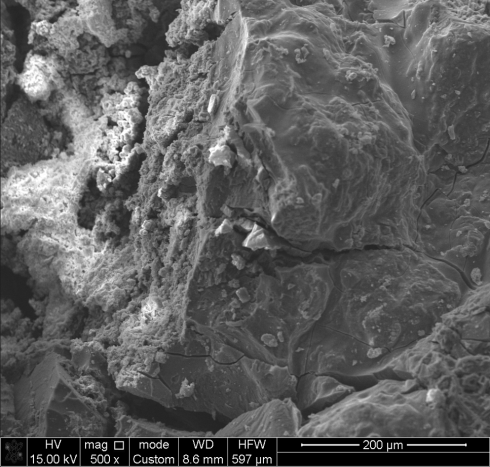
\includegraphics[width=0.8\textwidth]{media/chem2/image9}
	\caption*{}
\end{figure}

%% \end{minipage} & \begin{minipage}[b]{\linewidth}\centering
%% 
\begin{figure}[H]
	\centering
	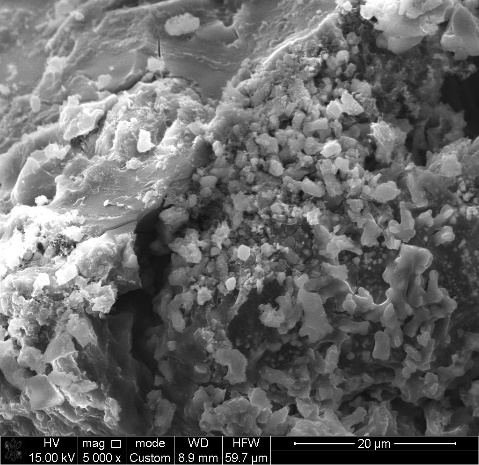
\includegraphics[width=0.8\textwidth]{media/chem2/image10}
	\caption*{}
\end{figure}

%% \end{minipage} & \begin{minipage}[b]{\linewidth}\centering
%% 
\begin{figure}[H]
	\centering
	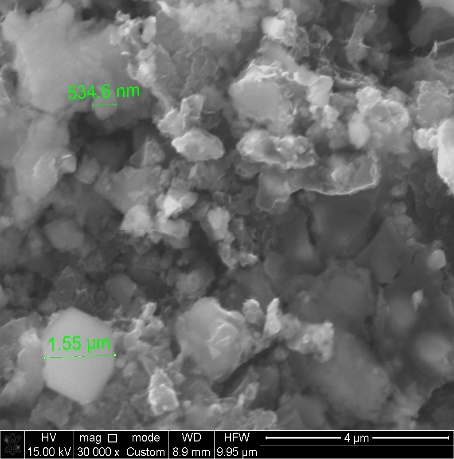
\includegraphics[width=0.8\textwidth]{media/chem2/image11}
	\caption*{}
\end{figure}

%% \end{minipage} \\
%% \midrule\noalign{}
%% \endhead
%% \bottomrule\noalign{}
%% \endlastfoot
%% a & b & c \\
%% \end{longtable}

{\bfseries Fig.1 - SEM results for the powdered activated adsorbent
"Shubarkol-KOH" (1:0.5, 900°C):}

{\bfseries а-х500; b-х5000; c-х30000}

%% \begin{longtable}[]{@{}
%%   >{\centering\arraybackslash}p{(\linewidth - 4\tabcolsep) * \real{0.3372}}
%%   >{\centering\arraybackslash}p{(\linewidth - 4\tabcolsep) * \real{0.3258}}
%%   >{\centering\arraybackslash}p{(\linewidth - 4\tabcolsep) * \real{0.3371}}@{}}
%% \toprule\noalign{}
%% \begin{minipage}[b]{\linewidth}\centering
%% 
\begin{figure}[H]
	\centering
	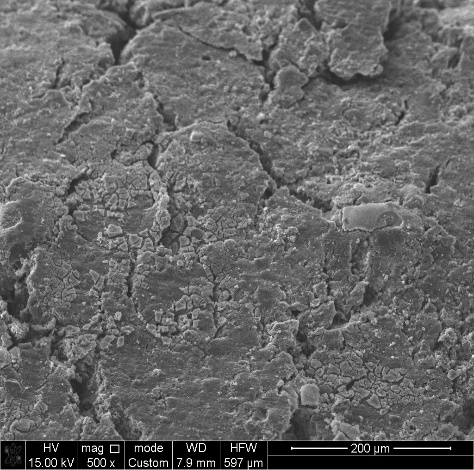
\includegraphics[width=0.8\textwidth]{media/chem2/image12}
	\caption*{}
\end{figure}

%% \end{minipage} & \begin{minipage}[b]{\linewidth}\centering
%% 
\begin{figure}[H]
	\centering
	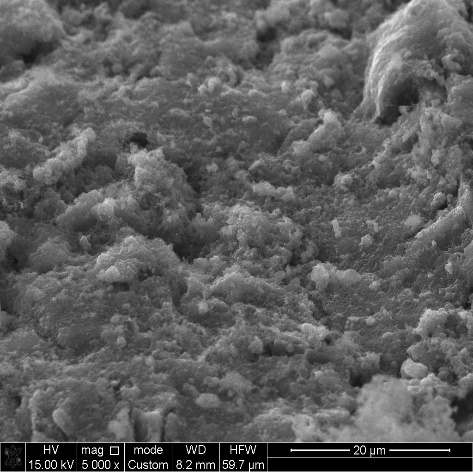
\includegraphics[width=0.8\textwidth]{media/chem2/image13}
	\caption*{}
\end{figure}

%% \end{minipage} & \begin{minipage}[b]{\linewidth}\centering
%% 
\begin{figure}[H]
	\centering
	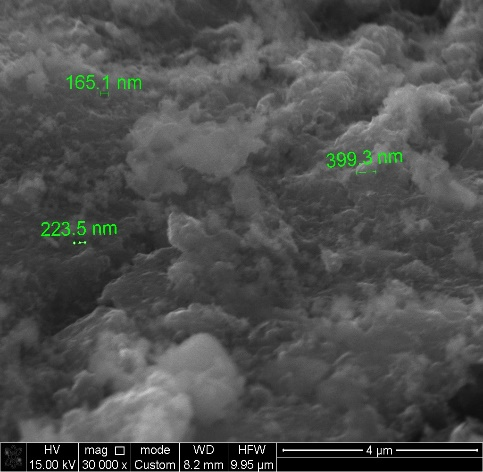
\includegraphics[width=0.8\textwidth]{media/chem2/image14}
	\caption*{}
\end{figure}

%% \end{minipage} \\
%% \midrule\noalign{}
%% \endhead
%% \bottomrule\noalign{}
%% \endlastfoot
%% a & b & c \\
%% \end{longtable}

{\bfseries Fig.2 - SEM results for the extruded activated adsorbent
"Shubarkol-KOH" (1:0.5, 900°C):}

{\bfseries а-х500; b-х5000; c-х30000}

The morphological analysis of the obtained adsorbents revealed that the
particle sizes of the surface of the adsorbents ranged from 534.6 nm to
1.55 µm for the powdered activated adsorbent "Shubarkol-KOH" (1:0.5,
900°C), and from 165.1 nm to 399.3 nm for the extruded activated
adsorbent "Shubarkol-KOH" (1:0.5, 900°C), exhibiting a heterogeneous
structure.

Figures 3 and 4 present the SEM analysis results for the powdered
activated adsorbent "Shoptykol-KOH" (1:0.5, 900°C) and the extruded
activated adsorbent "Shoptykol-KOH" (1:0.5, 900°C).

%% \begin{longtable}[]{@{}
%%   >{\centering\arraybackslash}p{(\linewidth - 4\tabcolsep) * \real{0.3372}}
%%   >{\centering\arraybackslash}p{(\linewidth - 4\tabcolsep) * \real{0.3258}}
%%   >{\centering\arraybackslash}p{(\linewidth - 4\tabcolsep) * \real{0.3371}}@{}}
%% \toprule\noalign{}
%% \begin{minipage}[b]{\linewidth}\centering
%% 
\begin{figure}[H]
	\centering
	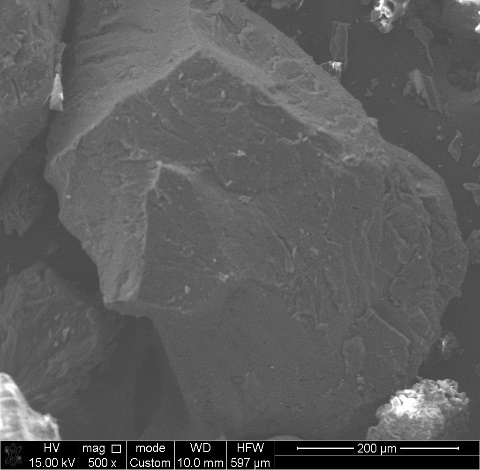
\includegraphics[width=0.8\textwidth]{media/chem2/image15}
	\caption*{}
\end{figure}

%% \end{minipage} & \begin{minipage}[b]{\linewidth}\centering
%% 
\begin{figure}[H]
	\centering
	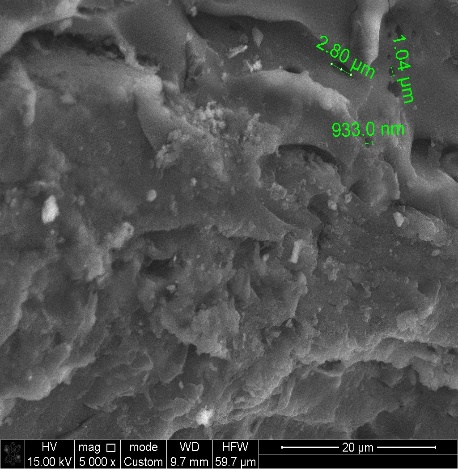
\includegraphics[width=0.8\textwidth]{media/chem2/image16}
	\caption*{}
\end{figure}

%% \end{minipage} & \begin{minipage}[b]{\linewidth}\centering
%% 
\begin{figure}[H]
	\centering
	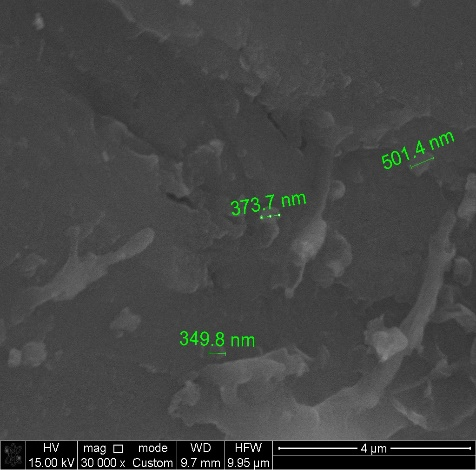
\includegraphics[width=0.8\textwidth]{media/chem2/image17}
	\caption*{}
\end{figure}

%% \end{minipage} \\
%% \midrule\noalign{}
%% \endhead
%% \bottomrule\noalign{}
%% \endlastfoot
%% а & b & c \\
%% \end{longtable}

{\bfseries Fig.3 - SEM results for the powdered activated adsorbent
"Shoptykol-KOH" (1:0.5, 900°C):}

{\bfseries а-х500; b-х5000; c-х30000}

%% \begin{longtable}[]{@{}
%%   >{\centering\arraybackslash}p{(\linewidth - 4\tabcolsep) * \real{0.3372}}
%%   >{\centering\arraybackslash}p{(\linewidth - 4\tabcolsep) * \real{0.3258}}
%%   >{\centering\arraybackslash}p{(\linewidth - 4\tabcolsep) * \real{0.3371}}@{}}
%% \toprule\noalign{}
%% \begin{minipage}[b]{\linewidth}\centering
%% 
\begin{figure}[H]
	\centering
	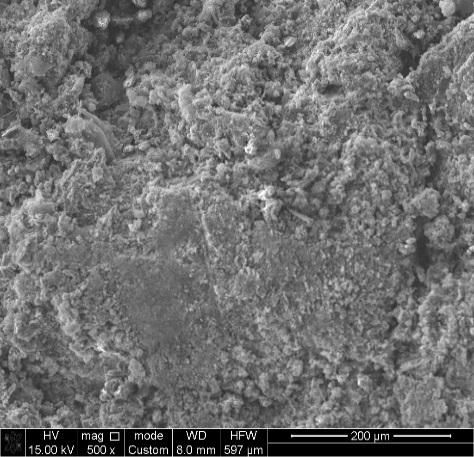
\includegraphics[width=0.8\textwidth]{media/chem2/image18}
	\caption*{}
\end{figure}

%% \end{minipage} & \begin{minipage}[b]{\linewidth}\centering
%% 
\begin{figure}[H]
	\centering
	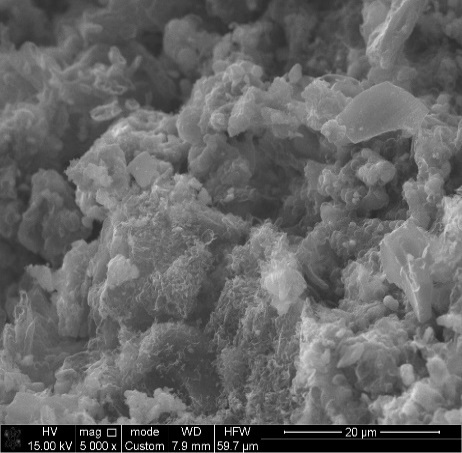
\includegraphics[width=0.8\textwidth]{media/chem2/image19}
	\caption*{}
\end{figure}

%% \end{minipage} & \begin{minipage}[b]{\linewidth}\centering
%% 
\begin{figure}[H]
	\centering
	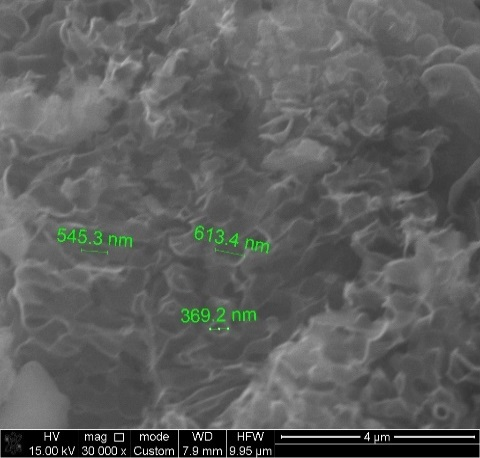
\includegraphics[width=0.8\textwidth]{media/chem2/image20}
	\caption*{}
\end{figure}

%% \end{minipage} \\
%% \midrule\noalign{}
%% \endhead
%% \bottomrule\noalign{}
%% \endlastfoot
%% а & b & c \\
%% \end{longtable}

{\bfseries Fig.4 - SEM results for the extruded activated adsorbent
"Shoptykol-KOH" (1:0.5, 900°C):}

{\bfseries а-х500; b-х5000; c-х30000}

The morphological analysis of the obtained adsorbents revealed that the
particle sizes of the surface of the adsorbents ranged from 349.8 nm to
501.4 nm for the powdered activated adsorbent "Shoptykol-KOH" (1:0.5,
900°C), and from 369.2 nm to 613.4 nm for the extruded activated
adsorbent "Shoptykol-KOH" (1:0.5, 900°C), both exhibiting a
heterogeneous structure.

The results of the elemental composition and physicochemical
characteristics of the samples are presented in Tables 1 and 2.

{\bfseries Table 1 - Results of the elemental analysis of the samples}

%% \begin{longtable}[]{@{}
%%   >{\centering\arraybackslash}p{(\linewidth - 20\tabcolsep) * \real{0.2601}}
%%   >{\centering\arraybackslash}p{(\linewidth - 20\tabcolsep) * \real{0.0877}}
%%   >{\centering\arraybackslash}p{(\linewidth - 20\tabcolsep) * \real{0.0738}}
%%   >{\centering\arraybackslash}p{(\linewidth - 20\tabcolsep) * \real{0.0732}}
%%   >{\centering\arraybackslash}p{(\linewidth - 20\tabcolsep) * \real{0.0733}}
%%   >{\centering\arraybackslash}p{(\linewidth - 20\tabcolsep) * \real{0.0624}}
%%   >{\centering\arraybackslash}p{(\linewidth - 20\tabcolsep) * \real{0.0624}}
%%   >{\centering\arraybackslash}p{(\linewidth - 20\tabcolsep) * \real{0.0732}}
%%   >{\centering\arraybackslash}p{(\linewidth - 20\tabcolsep) * \real{0.0733}}
%%   >{\centering\arraybackslash}p{(\linewidth - 20\tabcolsep) * \real{0.0875}}
%%   >{\centering\arraybackslash}p{(\linewidth - 20\tabcolsep) * \real{0.0732}}@{}}
%% \toprule\noalign{}
%% \multirow{2}{=}{\begin{minipage}[b]{\linewidth}\centering
%% Name
%% \end{minipage}} &
%% \multicolumn{10}{>{\centering\arraybackslash}p{(\linewidth - 20\tabcolsep) * \real{0.7399} + 18\tabcolsep}@{}}{%
%% \begin{minipage}[b]{\linewidth}\centering
%% Elemental content, mass \%
%% \end{minipage}} \\
%% & \begin{minipage}[b]{\linewidth}\centering
%% C
%% \end{minipage} & \begin{minipage}[b]{\linewidth}\centering
%% O
%% \end{minipage} & \begin{minipage}[b]{\linewidth}\centering
%% Na
%% \end{minipage} & \begin{minipage}[b]{\linewidth}\centering
%% Mg
%% \end{minipage} & \begin{minipage}[b]{\linewidth}\centering
%% Al
%% \end{minipage} & \begin{minipage}[b]{\linewidth}\centering
%% Si
%% \end{minipage} & \begin{minipage}[b]{\linewidth}\centering
%% S
%% \end{minipage} & \begin{minipage}[b]{\linewidth}\centering
%% K
%% \end{minipage} & \begin{minipage}[b]{\linewidth}\centering
%% Ca
%% \end{minipage} & \begin{minipage}[b]{\linewidth}\centering
%% Fe
%% \end{minipage} \\
%% \midrule\noalign{}
%% \endhead
%% \bottomrule\noalign{}
%% \endlastfoot
%% "Shubarkol-KOH" (1:0.5, 900°C) the powdered activated adsorbent & 71.15
%% & 11.78 & 1.94 & 0.49 & 9.57 & 0.19 & 0.11 & 1.33 & 1.12 & 2.31 \\
%% "Shubarkol-KOH" (1:0.5, 900°C) extruded activated adsorbent & 89.61 &
%% 8.11 & 0.08 & 0.04 & 0.44 & 0.96 & 0.01 & 0.48 & 0.10 & 0.17 \\
%% "Shoptykol-KOH" (1:0.5, 900°C) the powdered activated adsorbent & 88.19
%% & 7.60 & 0.15 & 0.40 & 0.11 & 0.15 & 0.24 & 0.73 & 1.65 & 0.77 \\
%% "Shoptykol-KOH" (1:0.5, 900°C) extruded activated adsorbent & 78.87 &
%% 10.79 & 0.08 & 0.13 & 1.87 & 3.16 & 0.17 & 3.25 & 0.97 & 0.70 \\
%% \end{longtable}

At elevated temperatures, potassium hydroxide reacts with carbon,
leading to the formation of gaseous carbon oxides. This reaction
promotes the development of a porous structure within the carbon
material and increases its surface area. Additionally, the reduction of
metal ions intercalated between carbon layers to their metallic state is
observed. Subsequent treatment with water further contributes to the
formation of pores. It is also important to note that during the
activation process with potassium hydroxide, inorganic components,
particularly silicon, form water-soluble potassium silicates. This
results in a reduction of ash content following activation and washing.

Elemental analysis indicates that the relatively highest carbon content
was observed in the extruded activated adsorbent "Shubarkol-KOH" (1:0.5,
900°C) and the powdered activated adsorbent "Shoptykol-KOH" (1:0.5,
900°C).

{\bfseries Table 2 - Characteristics of adsorbents obtained from coal from
the "Shubarkol" and "Shoptykol" deposits}

%% \begin{longtable}[]{@{}
%%   >{\centering\arraybackslash}p{(\linewidth - 18\tabcolsep) * \real{0.2827}}
%%   >{\centering\arraybackslash}p{(\linewidth - 18\tabcolsep) * \real{0.0596}}
%%   >{\centering\arraybackslash}p{(\linewidth - 18\tabcolsep) * \real{0.0744}}
%%   >{\centering\arraybackslash}p{(\linewidth - 18\tabcolsep) * \real{0.0745}}
%%   >{\centering\arraybackslash}p{(\linewidth - 18\tabcolsep) * \real{0.0745}}
%%   >{\centering\arraybackslash}p{(\linewidth - 18\tabcolsep) * \real{0.0894}}
%%   >{\centering\arraybackslash}p{(\linewidth - 18\tabcolsep) * \real{0.1044}}
%%   >{\centering\arraybackslash}p{(\linewidth - 18\tabcolsep) * \real{0.0744}}
%%   >{\centering\arraybackslash}p{(\linewidth - 18\tabcolsep) * \real{0.0895}}
%%   >{\centering\arraybackslash}p{(\linewidth - 18\tabcolsep) * \real{0.0765}}@{}}
%% \toprule\noalign{}
%% \begin{minipage}[b]{\linewidth}\centering
%% Name of activated adsorbent
%% \end{minipage} & \begin{minipage}[b]{\linewidth}\centering
%% \emph{W\textsuperscript{r}\textsubscript{t}},\%
%% \end{minipage} & \begin{minipage}[b]{\linewidth}\centering
%% \emph{A\textsuperscript{r}},\%
%% \end{minipage} & \begin{minipage}[b]{\linewidth}\centering
%% \emph{V\textsuperscript{d}}, \%
%% \end{minipage} & \begin{minipage}[b]{\linewidth}\centering
%% \emph{V}\textsubscript{Σ (water),} cm\textsuperscript{3}/g
%% \end{minipage} & \begin{minipage}[b]{\linewidth}\centering
%% ρ\textsubscript{bulk}, g/cm\textsuperscript{3}
%% \end{minipage} & \begin{minipage}[b]{\linewidth}\centering
%% рН\textsubscript{aqueous extract}
%% \end{minipage} & \begin{minipage}[b]{\linewidth}\centering
%% \emph{А\textsubscript{m.o.}},
%% 
%% mg/g
%% \end{minipage} & \begin{minipage}[b]{\linewidth}\centering
%% \emph{А\textsubscript{m.b.}}, mg/g
%% \end{minipage} & \begin{minipage}[b]{\linewidth}\centering
%% \emph{А}\textsubscript{iodine}, \%
%% \end{minipage} \\
%% \midrule\noalign{}
%% \endhead
%% \bottomrule\noalign{}
%% \endlastfoot
%% "Shubarkol-KOH" (1:0.5, 900°C) the powdered activated adsorbent & 25.14
%% & 8.65 & 52.95 & 0.54 & 0.51 & 7.01 & 30.1 & 44.4 & 34.54 \\
%% "Shubarkol-KOH" (1:0.5, 900°C) extruded activated adsorbent & 10.83 &
%% 21.44 & 62.61 & 0.56 & 0.62 & 7.37 & 52.0 & 89.8 & 31.42 \\
%% "Shoptykol-KOH" (1:0.5, 900°C) the powdered activated adsorbent & 8.66 &
%% 20.45 & 54.09 & 0.61 & 0.48 & 7.52 & 24.2 & 45.4 & 38.72 \\
%% "Shoptykol-KOH" (1:0.5, 900°C) extruded activated adsorbent & 16.81 &
%% 45.41 & 138.75 & 0.72 & 0.54 & 7.25 & 68.5 & 87.5 & 30.86 \\
%% \end{longtable}

In terms of methyl orange adsorption, the Shoptykol-KOH extruded
adsorbent demonstrated the highest capacity (68.5 mg/g). For methylene
blue, the best performance was observed for the Shubarkol-KOH extruded
adsorbent (89.8 mg/g), indicating its high sorption capacity for large
molecular weight dyes. Regarding iodine adsorption, the highest capacity
was found in the Shoptykol-KOH powdered adsorbent (38.72 mg/g),
suggesting a well-developed microporous structure.

Extruded adsorbents generally exhibited higher efficiency in removing
organic dyes, particularly methylene blue. Shoptykol-based adsorbents
showed superior adsorption of iodine, indicating a more developed
microporous structure. The choice of adsorbent should depend on the
target application: Shubarkol-KOH (extruded) is more effective for dye
removal, while Shoptykol-KOH (powdered) is better suited for the
adsorption of small molecules such as iodine.

{\bfseries Table 3- Specific surface area values \hspace{0pt}\hspace{0pt}of
pores of adsorbents obtained from coal from the "Shubarkol" and
"Shoptykol" deposits}

%% \begin{longtable}[]{@{}
%%   >{\centering\arraybackslash}p{(\linewidth - 8\tabcolsep) * \real{0.3425}}
%%   >{\centering\arraybackslash}p{(\linewidth - 8\tabcolsep) * \real{0.1348}}
%%   >{\centering\arraybackslash}p{(\linewidth - 8\tabcolsep) * \real{0.1941}}
%%   >{\centering\arraybackslash}p{(\linewidth - 8\tabcolsep) * \real{0.1792}}
%%   >{\centering\arraybackslash}p{(\linewidth - 8\tabcolsep) * \real{0.1494}}@{}}
%% \toprule\noalign{}
%% \begin{minipage}[b]{\linewidth}\centering
%% Name of activated adsorbent
%% \end{minipage} & \begin{minipage}[b]{\linewidth}\centering
%% BET Surface Area, m\textsuperscript{2}/a
%% \end{minipage} & \begin{minipage}[b]{\linewidth}\centering
%% Cumulative adsorption surface area (BJH) for pores with a width from
%% 17,000 Å to 3,000,000 Å, m²/g
%% \end{minipage} & \begin{minipage}[b]{\linewidth}\centering
%% BJH adsorption cumulative pore volume for pores with a width from 17,000
%% Å to 3,000,000 Å, cm³/g
%% \end{minipage} & \begin{minipage}[b]{\linewidth}\centering
%% BJH adsorption average pore width (4V/A), Å
%% \end{minipage} \\
%% \midrule\noalign{}
%% \endhead
%% \bottomrule\noalign{}
%% \endlastfoot
%% "Shubarkol-KOH" (1:0.5, 900°C) the powdered activated adsorbent &
%% 507.2986 & 59.4994 & 0.12044 & 80.972 \\
%% "Shubarkol-KOH" (1:0.5, 900°C) extruded activated adsorbent & 316.8146 &
%% 62.64589 & 0.09226 & 21.372 \\
%% "Shoptykol-KOH" (1:0.5, 900°C) the powdered activated adsorbent &
%% 926.6728 & 130.0567 & 0.13067 & 40.191 \\
%% "Shoptykol-KOH" (1:0.5, 900°C) extruded activated adsorbent & 381.3587 &
%% 123.41338 & 0.14172 & 21.459 \\
%% \end{longtable}

Figure 5 shows the BET isotherm of the specific surface area of the
extruded activated adsorbents "Shubarkol-KOH" (1:0.5, 900°C) and
"Shoptykol-KOH" (1:0.5, 900°C).

%% \begin{longtable}[]{@{}
%%   >{\centering\arraybackslash}p{(\linewidth - 2\tabcolsep) * \real{0.4914}}
%%   >{\centering\arraybackslash}p{(\linewidth - 2\tabcolsep) * \real{0.5086}}@{}}
%% \toprule\noalign{}
%% \begin{minipage}[b]{\linewidth}\raggedright
%% 
\begin{figure}[H]
	\centering
	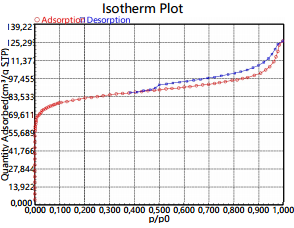
\includegraphics[width=0.8\textwidth]{media/chem2/image21}
	\caption*{}
\end{figure}

%% \end{minipage} & \begin{minipage}[b]{\linewidth}\raggedright
%% 
\begin{figure}[H]
	\centering
	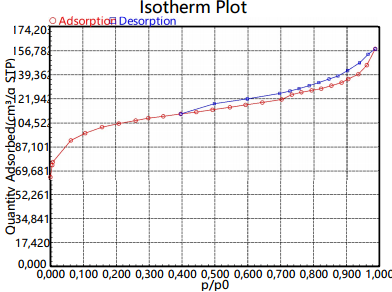
\includegraphics[width=0.8\textwidth]{media/chem2/image22}
	\caption*{}
\end{figure}

%% \end{minipage} \\
%% \midrule\noalign{}
%% \endhead
%% \bottomrule\noalign{}
%% \endlastfoot
%% a & b \\
%% \end{longtable}

{\bfseries Fig.5 -- BET isotherm of the specific surface area of the
extruded activated adsorbent (a -- "Shubarkol-KOH" 1:0.5, 900°C, b --
"Shoptykol-KOH" 1:0.5, 900°C)}

Figure 6 shows the types of adsorption-desorption isotherms.


\begin{figure}[H]
	\centering
	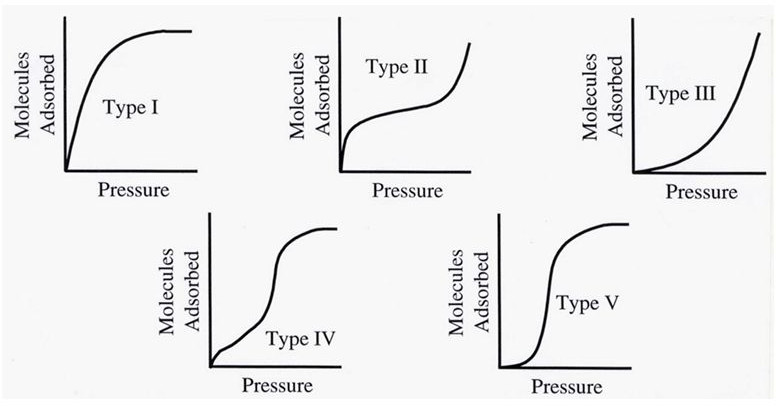
\includegraphics[width=0.8\textwidth]{media/chem2/image23}
	\caption*{}
\end{figure}


{\bfseries Fig.6 -- Types of adsorption-desorption isotherms}

The types of adsorption-desorption isotherms of the obtained adsorbents
were determined, and conclusions were drawn. The adsorption-desorption
isotherms of the mesopores of the "Shubarkol-KOH" (1:0.5, 900°C)
extruded activated adsorbent and the "Shoptykol-KOH" (1:0.5, 900°C)
extruded activated adsorbent correspond to Type I and Type II isotherms.

Type I -- "Langmuir-type" isotherm is characterized by the cessation of
adsorption growth at low and medium relative pressures. This type of
isotherm occurs in two cases:

During monomolecular adsorption on macroporous adsorbents, where strong
adsorbate-adsorbent interactions are observed.

During adsorption in microporous adsorbents. Unlike the first case, in
the presence of micropores, a sharp increase is observed at low relative
pressure values (p/p\textsubscript{s} \textless{} 0.1), which is due to
the high adsorption potential. Additionally, the specific surface area
of microporous samples significantly exceeds that of macroporous or
non-porous materials.

Type II -- "S-shaped" isotherm indicates the formation of polymolecular
adsorption. Typically, this form of isotherm is characteristic of
dispersed macroporous and non-porous materials.

%% \begin{longtable}[]{@{}
%%   >{\centering\arraybackslash}p{(\linewidth - 2\tabcolsep) * \real{0.5093}}
%%   >{\centering\arraybackslash}p{(\linewidth - 2\tabcolsep) * \real{0.4907}}@{}}
%% \toprule\noalign{}
%% \begin{minipage}[b]{\linewidth}\raggedright
%% 
\begin{figure}[H]
	\centering
	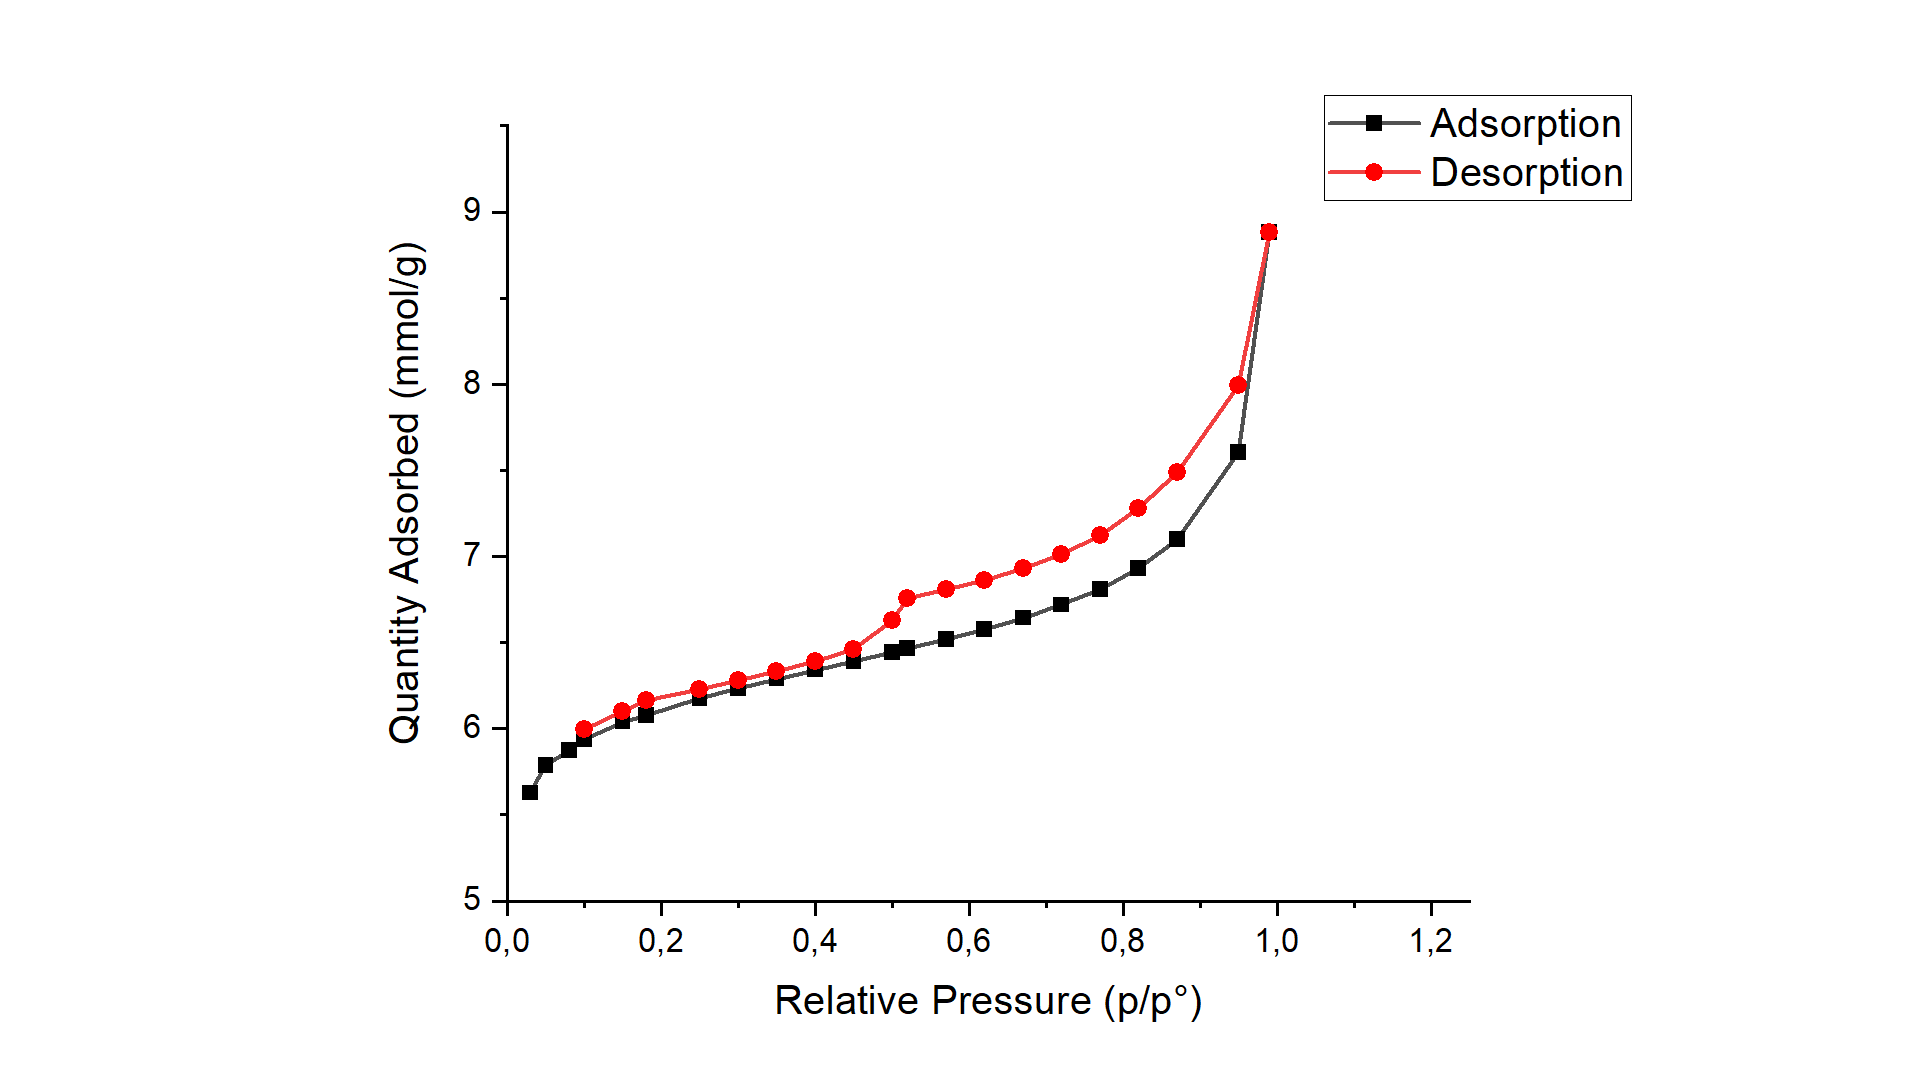
\includegraphics[width=0.8\textwidth]{media/chem2/image24}
	\caption*{}
\end{figure}

%% \end{minipage} & \begin{minipage}[b]{\linewidth}\raggedright
%% 
\begin{figure}[H]
	\centering
	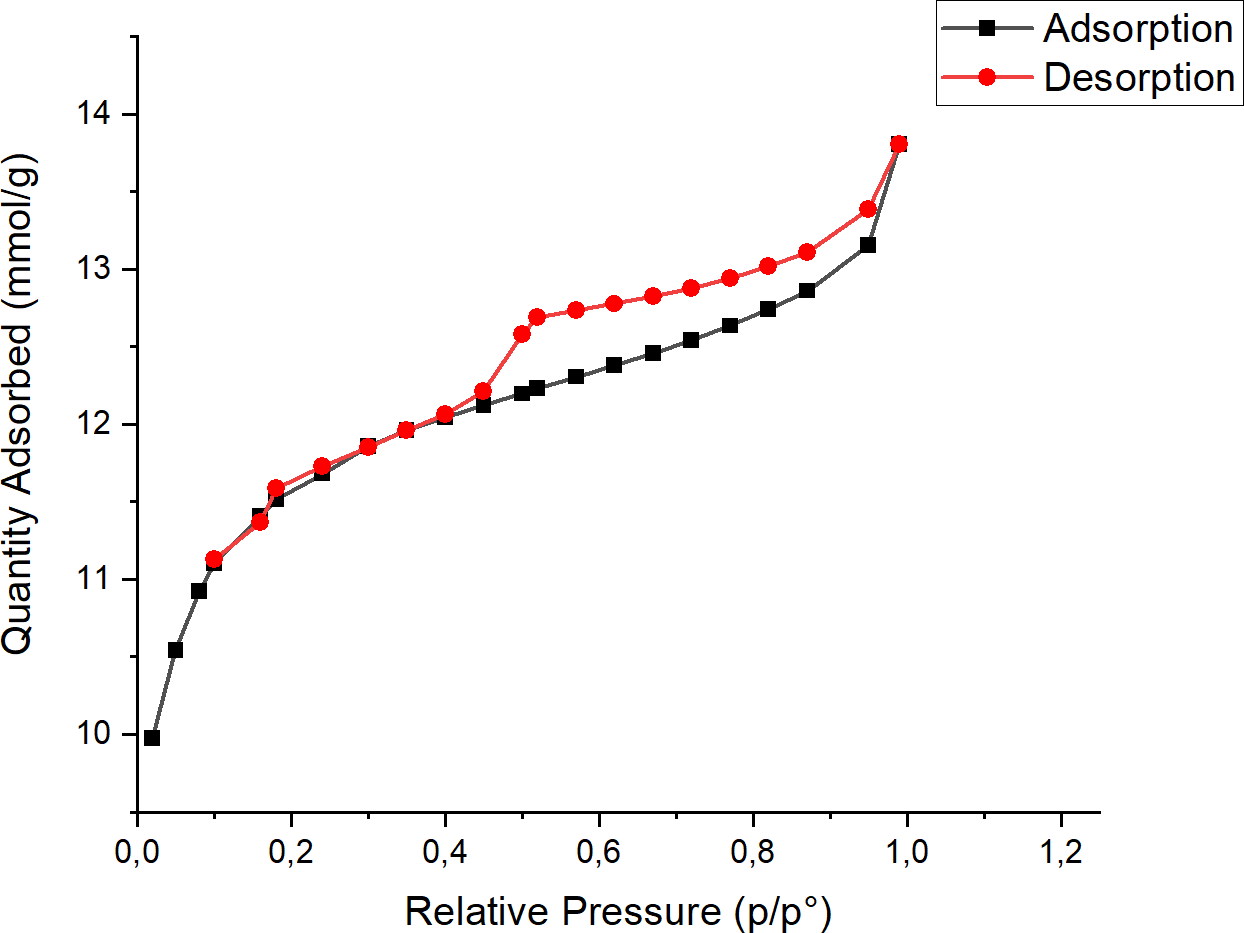
\includegraphics[width=0.8\textwidth]{media/chem2/image25}
	\caption*{}
\end{figure}

%% \end{minipage} \\
%% \midrule\noalign{}
%% \endhead
%% \bottomrule\noalign{}
%% \endlastfoot
%% a & b \\
%% \end{longtable}

{\bfseries Fig.7 -- BET isotherm of the specific surface area of the
powdered activated adsorbent (a -- "Shubarkol-KOH" 1:0.5, 900°C, b --
"Shoptykol-KOH" 1:0.5, 900°C)}

The obtained isotherms of the samples belong to type I - a microporous
material; there is also a type IV hysteresis loop, also characteristic
of a microporous material with slot-like pores, characteristic of the
layered structure of coals.

Among the powdered activated adsorbents, "Shoptykol-KOH" (1:0.5, 900°C)
exhibits the highest BET surface area (926.67 m²/g), significantly
higher than "Shubarkol-KOH" (507.30 m²/g). Among the extruded activated
adsorbents, "Shoptykol-KOH" (381.36 m²/g) again outperforms
"Shubarkol-KOH" (316.81 m²/g) in terms of specific surface area. In both
cases, the powdered form of the adsorbents shows a higher surface area
than the extruded form, indicating that pelletization may lead to some
loss of porosity.

"Shoptykol-KOH" (1:0.5, 900°C) powdered activated adsorbent demonstrates
the highest BET surface area (926.67 m²/g), which is a critical factor
for gas adsorption. The hydrogen storage capacity of this adsorbent is
77\% with a K-value of 1.48, indicating strong potential for hydrogen
adsorption. A higher surface area typically correlates with improved
hydrogen uptake due to enhanced microporosity and available adsorption
sites.


\begin{figure}[H]
	\centering
	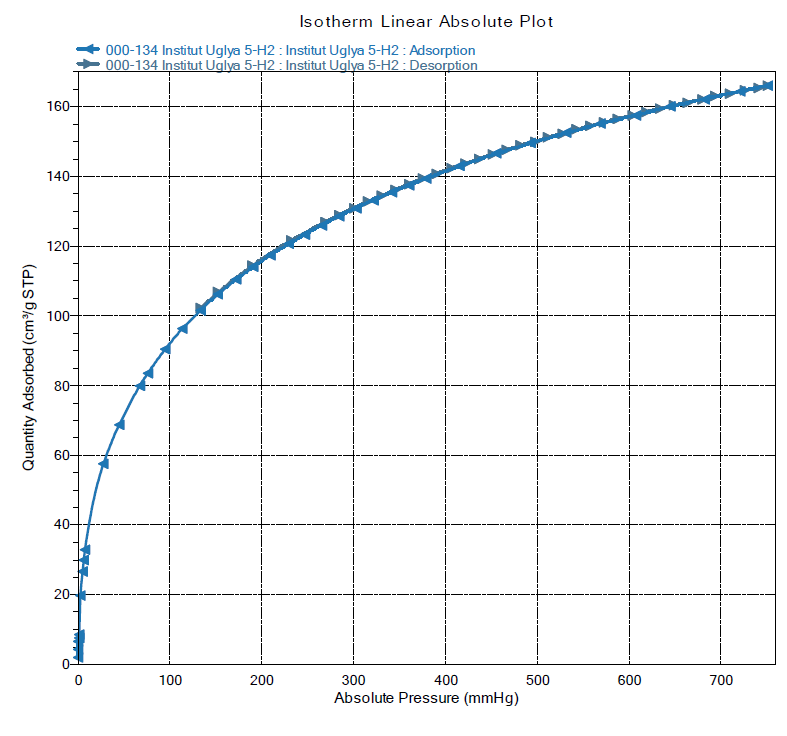
\includegraphics[width=0.8\textwidth]{media/chem2/image26}
	\caption*{}
\end{figure}


{\bfseries Fig.8- Adsorption curve of the powdered activated adsorbent
"Shoptykol:KOH" 1:0.5, 900ºC (H\textsubscript{2})}

Hydrogen sorption was carried out at 3 different temperatures.

{\bfseries Table 4 - Results of the study of hydrogen sorption with PСM}

%% \begin{longtable}[]{@{}
%%   >{\centering\arraybackslash}p{(\linewidth - 10\tabcolsep) * \real{0.1813}}
%%   >{\centering\arraybackslash}p{(\linewidth - 10\tabcolsep) * \real{0.1898}}
%%   >{\centering\arraybackslash}p{(\linewidth - 10\tabcolsep) * \real{0.1438}}
%%   >{\centering\arraybackslash}p{(\linewidth - 10\tabcolsep) * \real{0.1668}}
%%   >{\centering\arraybackslash}p{(\linewidth - 10\tabcolsep) * \real{0.1364}}
%%   >{\centering\arraybackslash}p{(\linewidth - 10\tabcolsep) * \real{0.1819}}@{}}
%% \toprule\noalign{}
%% \begin{minipage}[b]{\linewidth}\centering
%% Name
%% \end{minipage} & \begin{minipage}[b]{\linewidth}\centering
%% S(\textsubscript{DFT}) specific, m\textsuperscript{2}/g
%% \end{minipage} & \begin{minipage}[b]{\linewidth}\centering
%% Mass H\textsubscript{2}, \% 77 K
%% \end{minipage} & \begin{minipage}[b]{\linewidth}\centering
%% Mass H\textsubscript{2}, \% 273 K
%% \end{minipage} & \begin{minipage}[b]{\linewidth}\centering
%% Mass H\textsubscript{2}, \%
%% 
%% 298 K
%% \end{minipage} & \begin{minipage}[b]{\linewidth}\centering
%% Heat of adsorption of H\textsubscript{2}, kJ/mol
%% \end{minipage} \\
%% \midrule\noalign{}
%% \endhead
%% \bottomrule\noalign{}
%% \endlastfoot
%% Shoptykol:
%% 
%% KOH = 1:0.5 & 1184,29 & 1,48 & 0.021 & 0.0084 & 17,31 \\
%% \end{longtable}

For the case of 77 K, it is also possible to determine the specific
surface area and pore distribution using DFT methods for carbon
materials. Unfortunately, the method has not been developed for other
temperatures and heterogeneous surfaces which these samples belong to.
As logically follows, an increase in temperature significantly reduces
the sorption of hydrogen. From the capacitance values
\hspace{0pt}\hspace{0pt}obtained at 3 different temperatures, the heat
of adsorption of hydrogen molecules can be determined.

A comparison table comparing the specific surface area
S(\textsubscript{BET}) for N\textsubscript{2}, CO\textsubscript{2} and
H\textsubscript{2} is presented in Table 5.

{\bfseries Table 5 - Comparative table comparing the specific surface area
S(\textsubscript{BET}) for N\textsubscript{2}, CO\textsubscript{2} and
H\textsubscript{2}}

%% \begin{longtable}[]{@{}
%%   >{\centering\arraybackslash}p{(\linewidth - 14\tabcolsep) * \real{0.0973}}
%%   >{\centering\arraybackslash}p{(\linewidth - 14\tabcolsep) * \real{0.1375}}
%%   >{\centering\arraybackslash}p{(\linewidth - 14\tabcolsep) * \real{0.1339}}
%%   >{\centering\arraybackslash}p{(\linewidth - 14\tabcolsep) * \real{0.1340}}
%%   >{\centering\arraybackslash}p{(\linewidth - 14\tabcolsep) * \real{0.1489}}
%%   >{\centering\arraybackslash}p{(\linewidth - 14\tabcolsep) * \real{0.1191}}
%%   >{\centering\arraybackslash}p{(\linewidth - 14\tabcolsep) * \real{0.1171}}
%%   >{\centering\arraybackslash}p{(\linewidth - 14\tabcolsep) * \real{0.1122}}@{}}
%% \toprule\noalign{}
%% \multirow{2}{=}{\begin{minipage}[b]{\linewidth}\centering
%% Temperature, K
%% \end{minipage}} &
%% \multirow{2}{=}{\begin{minipage}[b]{\linewidth}\centering
%% S(\textsubscript{BET}), m\textsuperscript{2}/g (based on
%% N\textsubscript{2})
%% \end{minipage}} &
%% \multicolumn{2}{>{\centering\arraybackslash}p{(\linewidth - 14\tabcolsep) * \real{0.2679} + 2\tabcolsep}}{%
%% \begin{minipage}[b]{\linewidth}\centering
%% Equivalent surface area (S), m²/g (based on CO\textsubscript{2})
%% \end{minipage}} &
%% \multirow{2}{=}{\begin{minipage}[b]{\linewidth}\centering
%% Specific surface S\textsubscript{(DFT)}, m\textsuperscript{2}/g
%% (according to H\textsubscript{2})
%% \end{minipage}} &
%% \multicolumn{2}{>{\centering\arraybackslash}p{(\linewidth - 14\tabcolsep) * \real{0.2362} + 2\tabcolsep}}{%
%% \begin{minipage}[b]{\linewidth}\centering
%% Amount of adsorbed H\textsubscript{2} gas
%% \end{minipage}} &
%% \multirow{2}{=}{\begin{minipage}[b]{\linewidth}\centering
%% Heat of adsorption of H\textsubscript{2}, kJ/mol
%% \end{minipage}} \\
%% & & \begin{minipage}[b]{\linewidth}\centering
%% Dubinin-Radushkevich
%% \end{minipage} & \begin{minipage}[b]{\linewidth}\centering
%% Dubinin-Astakhov
%% \end{minipage} & & \begin{minipage}[b]{\linewidth}\centering
%% \%
%% \end{minipage} & \begin{minipage}[b]{\linewidth}\centering
%% mg/g
%% \end{minipage} \\
%% \midrule\noalign{}
%% \endhead
%% \bottomrule\noalign{}
%% \endlastfoot
%% \multicolumn{8}{@{}>{\centering\arraybackslash}p{(\linewidth - 14\tabcolsep) * \real{1.0000} + 14\tabcolsep}@{}}{%
%% Powdered activated adsorbent Shoptykol:KOH (1:0.5)
%% 900\textsuperscript{0}С} \\
%% 77 & 926,6728 & 706,124 & 1605,444 & 1184,29 & 1,48 & 14,8203 & 17,31 \\
%% 273,15 & - & - & - & - & 0,021 & 0,21024 & - \\
%% 298 & - & - & - & - & 0,0083 & 0,08570 & - \\
%% \end{longtable}

Due to the smaller radius and transverse radius of the hydrogen
molecule, the specific surface area and porosity values
\hspace{0pt}\hspace{0pt}will be higher compared to nitrogen sorption.
Classical BET methods in the case of H\textsubscript{2} will be
incorrect, since the saturation pressure value was used as a constant
(760 Torr) to calculate the pore distribution, the theoretical model of
hydrogen sorption DFT HS H\textsubscript{2} Carbon heterogeneous, taking
into account the heterogeneity of the carbon surface. For most samples,
this model showed good agreement; the nitrogen limitation to fill pores
with a radius of less than 0.35 nm was also taken into account. To
calculate the heat of adsorption in the case of hydrogen, the affinity
coefficient parameter was considered equal to 0.165 according to
{[}13{]}, for nitrogen β=0.33.

The change in specific surface area using the (BET) method for hydrogen
(\%) and the amount of adsorbed hydrogen versus temperature for
activated adsorbents are presented below in Figure 9,10.

{\bfseries Fig.9- Change in specific surface area using the (BET) method
for hydrogen (\%) from the temperature of the powdered activated
adsorbent "Shoptykol: KOH" (1:0.5) at 900ºC}

{\bfseries Fig.10 - Change in the amount of adsorbed hydrogen as a function
of temperature for the powdered activated adsorbent "Shoptykol: KOH"
(1:0.5) at 900ºC}

The data indicate that low temperatures (-200°C) are optimal for
maximizing both specific surface area and hydrogen adsorption capacity.
As the temperature increases, the surface area reduces, leading to a
significant decline in hydrogen adsorption efficiency.

{\bfseries Conclusion.} This study comprehensively investigated the
hydrogen sorption properties of activated carbon adsorbents derived from
coals from the Kazakhstan deposits "Shubarkol" and "Shoptykol." The
research focused on the effect of activation conditions, material
structure, and surface characteristics on hydrogen adsorption
efficiency. The findings demonstrate that the activation process using
KOH in a 1:0.5 ratio, followed by thermal treatment at 900°C,
significantly enhances the porous structure of the resulting carbon
materials, increasing their specific surface area and adsorption
capacity.

Among the obtained adsorbents, the powdered "Shoptykol-KOH" (1:0.5,
900°C) material exhibited the highest BET surface area (926.67 m²/g) and
the greatest hydrogen storage capacity (1.48 wt.\% at 77 K). The results
suggest that the porous carbon adsorbents prepared under these
conditions possess a well-developed microporous structure, which is
crucial for hydrogen adsorption through physisorption mechanisms. The
adsorption-desorption isotherm analysis further classified the materials
into Type I and Type II, indicating the presence of both microporous and
mesoporous structures, making them suitable for various gas storage
applications.

Temperature-dependent hydrogen sorption studies revealed a strong
correlation between adsorption efficiency and operating temperature.
Hydrogen uptake was maximized at cryogenic temperatures (77 K),
confirming that low temperatures significantly enhance adsorption due to
increased van der Waals interactions. However, at room temperature (298
K), the adsorption capacity dropped considerably, underscoring the
challenge of efficient hydrogen storage under ambient conditions.

In summary, the powdered "Shoptykol-KOH" (1:0.5, 900°C) adsorbent has
been identified as the most promising material for hydrogen storage due
to its high specific surface area, well-developed microporous structure,
and superior hydrogen adsorption capacity at low temperatures. These
findings contribute to the ongoing development of efficient and
sustainable hydrogen storage technologies. Future studies should focus
on optimizing activation conditions, exploring alternative activation
agents, and functionalizing the adsorbent surface to enhance hydrogen
uptake at ambient temperatures. Additionally, scaling up the production
of these materials and evaluating their long-term stability in
real-world hydrogen storage applications will be essential for their
commercial implementation.

\emph{{\bfseries Funding}.This research has been funded by the Science
Committee of the Ministry of Science and Higher Education of the
Republic of Kazakhstan (Grant No. AP19577512 "Development of scientific
and technical bases for obtaining microporous carbon nanomaterials for
hydrogen separation and storage").}

{\bfseries References}


1. Park J.H., Ramasamy P., Kim S., Kim Y.K., Ahilan V., Shanmugam S., Lee
J.S. Hybrid metal---Cu2S nanostructures as efficient co-catalysts for
photocatalytic hydrogen generation// Chem. Commun. -2017. - Vol.53
(22). - P.3277--3280. DOI 10.1039/C7CC00071E.

1. Moriarty, P.; Honnery, D. Hydrogen's role in an uncertain energy
future // Int. J. Hydrog. Energy. - 2009. Vol.34. -P.31 -39. DOI
\href{http://dx.doi.org/10.1016/j.ijhydene.2008.10.060}{10.1016/j.ijhydene.2008.10.060}.

1. Schlapbach, L.; Züttel, A. Hydrogen-storage materials for mobile
applications. Mater. Sustain //Energy. -2010. -P.265-270. DOI
\href{http://dx.doi.org/10.1142/9789814317665_0038}{10.1142/9789814317665\_0038}.

1. Dincer I. Environmental and sustainability aspects of hydrogen and
fuel cell systems. Int J Energy Res. -2007. - Vol.31(1). - P.29-55.
\href{https://doi.org/10.1002/er.1226}{DOI 10.1002/er.1226}.

1. Weinberger B, Lamari FD. High pressure cryo-storage of hydrogen by
adsorption at 77K and up to 50MPa // International Journal of Hydrogen
Energy. - 2009. - Vol.34(7). - P.3058-3064.
\href{https://doi.org/10.1016/j.ijhydene.2009.01.093}{DOI
10.1016/j.ijhydene.2009.01.093}.

1. Hwang S.-H., Kim Y. K., Seo H.-J., Jeong S. M., Kim J., Lim S. K. The
enhanced hydrogen storage capacity of carbon fibers: the effect of
hollow porous structure and surface modification // Nanomaterials. -
2021. - Vol.11(7). - 1830. DOI 10.3390/nano11071830.

1. Xia Y., Yang Z., Zhu Y. Porous carbon-based materials for hydrogen
storage: advancement and challenges // Journal of Materials Chemistry
A. - 2013. -Vol.1 (33). - P.9365-9381. DOI 10.1039/c3ta10583k.

1. Bader N., Ouederni A. Optimization of biomass-based carbon materials
for hydrogen storage // Journal of Energy Storage. - 2016. -Vol.5. -
P.77-84. \href{https://doi.org/10.1016/j.est.2015.12.009}{DOI
\href{http://dx.doi.org/10.1109/IREC.2015.7110967}{10.1109/IREC.2015.7110967}}.

1. Kopac T. Hydrogen storage characteristics of bio-based porous carbons
of different origin: A comparative review //
\href{https://onlinelibrary.wiley.com/journal/1099114x}{International
Journal of Energy Research}. - 2021. Vol.45(15). - P.20497-20523.
\href{https://doi.org/10.1002/er.7130}{DOI 10.1002/er.7130}.
10. Minoda A., Oshima S., Iki H., Akiba E. Synthesis of KOH-activated
porous carbon materials and study of hydrogen adsorption //
\href{https://www.researchgate.net/journal/Journal-of-Alloys-and-Compounds-0925-8388?_tp=eyJjb250ZXh0Ijp7ImZpcnN0UGFnZSI6InB1YmxpY2F0aW9uIiwicGFnZSI6InB1YmxpY2F0aW9uIn19}{Journal
of Alloys and Compounds}. - 2013. -Vol.580. - P. S301-S304.
\href{https://doi.org/10.1016/j.jallcom.2013.02.085}{DOI
10.1016/j.jallcom.2013.02.085}.

11. Zhang C., Geng Z, Cai M., et al. Microstructure regulation of super
activated carbon from biomass source corncob with enhanced hydrogen
uptake // International Journal of Hydrogen Energy. - 2013. -Vol.38(22).
- P.9243-9250.
\href{https://doi.org/10.1016/j.ijhydene.2013.04.163}{DOI
10.1016/j.ijhydene.2013.04.163}.

12. Dincer I, Acar C. Review and evaluation of hydrogen production
methods for better sustainability // International Journal of Hydrogen
Energy. - 2015. -Vol.40(34). - P.11094-11111.
\href{https://doi.org/10.1016/j.ijhydene.2014.12.035}{DOI
10.1016/j.ijhydene.2014.12.035}.

13. Rzepka M., Lamp P., de la Casa-Lillo M. A. Physisorbption of hydrogen
on Microporous Carbon and Carbon nanotubes // The Journal of Physical
Chemistry. - 1998. - Vol.102 (52). - P.10894-10898. DOI
10.1021/jp9829602.

\emph{{\bfseries Сведения об авторах}}

Казанкапова М.К. -- PhD, асс. профессор, чл.-корр. КазНАЕН, ведущий
научный сотрудник, заведующий лабораторией ТОО «Институт химии и
технологии угля», Астана, Казахстан, e-mail:
\href{mailto:maira_1986@mail.ru}{};

Ермагамбет Б.Т. -- доктор химических наук, профессор, академик КазНАЕН,
руководитель проекта, главный научный сотрудник, директор ТОО «Институт
химии и технологии угля», Астана, Казахстан, e-mail:


Касенова Ж.М. -- кандидат химических наук, заместитель директора ТОО
«Институт химии и технологии угля», Астана, Казахстан, e-mail:
\href{mailto:zhanar_k_68@mail.ru}{};

Малғаждарова А.Б. -- младший научный сотрудник ТОО «Институт химии угля
и технологии», магистрант Евразийского национального университета им.
Л.Н.Гумилева, Астана, Казахстан, e-mail:
\href{mailto:malgazhdarova.ab@mail.ru}{\nolinkurl{malgazhdarova.ab@mail.ru}};

Даулетжанова Ж.Т. -- доктор PhD, доцент Казахского университета
технологии и бизнеса имени К. Кулажанова, Астана, ведущий научный
сотрудник ТОО «Институт Химии угля и технологии», Астана, Казакстан
e-mail:
\href{mailto:kaliyeva_zhanna@mail.ru}{\nolinkurl{kaliyeva\_zhanna@mail.ru}};

Қожамұратова Ұ.М. - младший научный сотрудник ТОО «Институт химии угля и
технологии», магистрант Евразийского национального университета им.
Л.Н.Гумилева, Астана, Казахстан, e-mail:
\href{mailto:kozhamuratova.u@mail.ru}{\nolinkurl{kozhamuratova.u@mail.ru}};

Мендалиев Г.К. - младший научный сотрудник ТОО «Институт химии угля и
технологии», магистрант Евразийского национального университета им.
Л.Н.Гумилева, Астана, Казахстан, e-mail:
\href{mailto:ganimen02@mail.ru}{\nolinkurl{ganimen02@mail.ru}};

Акшекина Ә.С. - старший лаборант ТОО «Институт химии угля и технологии»,
магистрант Евразийского национального университета им. Л.Н.Гумилева,
Астана, Казахстан, e-mail:
\href{mailto:akshekina11@gmail.com}{\nolinkurl{akshekina11@gmail.com}}

\emph{{\bfseries Information about the authors}}

Kazankapova M.K. -- PhD in Philosophy, Associate Professor,
Corresponding Member of KazNAEN, Leading Researcher, Head of Laboratory
of LLP "Institute of Coal Chemistry and Technology", Astana, Kazakhstan,
e-mail: \href{mailto:maira_1986@mail.ru}{};

Yermagambet B.T. -- Doctor of Chemical Sciences, Professor, Academician
of KazNAEN, Project Manager, Chief Researcher, Director of LLP
"Institute of Coal Chemistry and Technology", Astana, Kazakhstan,
e-mail: \href{mailto:bake.yer@mail.ru}{};

Kassenova Zh.M. -- Candidate of Chemical Sciences, Deputy Director of
LLP "Institute of Coal Chemistry and Technology", Astana, Kazakhstan,
e-mail: \href{mailto:zhanar_k_68@mail.ru}{};

Malgazhdarova A.B. -- Junior Researcher of LLP «Institute of Coal
Chemistry and Technology», master student Eurasian National University
of L.N. Gumilyov, Astana, Kazakhstan, e-mail:
\href{mailto:malgazhdarova.ab@mail.ru}{\nolinkurl{malgazhdarova.ab@mail.ru}};
Dauletzhanova Zh. T. - PhD Doctor, Technology, Kazakh University of
Technology and Business named after K. Kulazhanov, Leading Researcher of
LLP "Institute of Coal Chemistry and Technology" Astana, Kazakhstan,
e-mail:
\href{mailto:kaliyeva_zhanna@mail.ru}{\nolinkurl{kaliyeva\_zhanna@mail.ru}};

Kozhamuratova U.M. -- Junior Researcher of LLP «Institute of Coal
Chemistry and Technology», master student Eurasian National University
of L.N. Gumilyov, Astana, Kazakhstan, e-mail:
\href{mailto:kozhamuratova.u@mail.ru}{\nolinkurl{kozhamuratova.u@mail.ru}};

Mendaliyev G. K. -- Junior Researcher of LLP «Institute of Coal
Chemistry and Technology», master student Eurasian National University
of L.N. Gumilyov, Astana, Kazakhstan, e-mail:
\href{mailto:ganimen02@mail.ru}{\nolinkurl{ganimen02@mail.ru}};

Akshekina A.S. -- Senior Lab Assistant of LLP «Institute of Coal
Chemistry and Technology», master student Eurasian National University
of L.N. Gumilyov, Astana, Kazakhstan, e-mail:
\href{mailto:akshekina11@gmail.com}{\nolinkurl{akshekina11@gmail.com}}\